%Folgende Zeile aktivieren und als SVN property "svn:keywords" auf "Id" setzen, um SVN Versionsinformationen im Dokument zu erhalten
%\svnInfo $Id: einleitung.tex 60 2012-01-26 15:56:06Z koppor $ 

\chapter{3D - Verfahren}
\label{chap:3d}
\subsection{RANSAC}
RANSAC (\textbf{RA}ndom \textbf{SA}mple \textbf{C}onsensus) ist ein iteratives Verfahren zur Schätzung eines mathematischen Models anhand von Beobachtungsdaten mit Ausreißern. Der Algorithmus ist nicht-deterministisch, da ihm probabilistische Ansätze zu Grund liegen. Aufgrund seiner Robustheit wird er häufig im Bereich des maschinellen Sehens eingesetzt. 

\begin{figure}[H]
  \begin{center}
    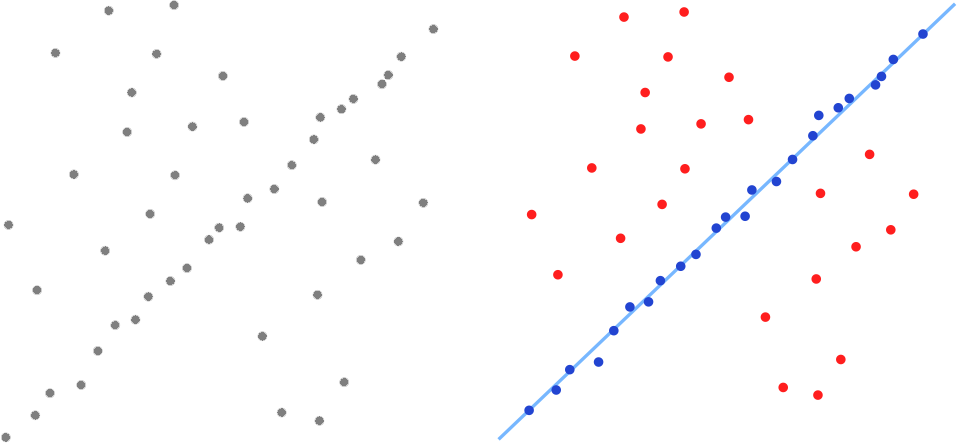
\includegraphics[width=0.9\textwidth]{RANSACline.png}
    \caption{In einen Datensatz mit vielen Ausreißern wird eine Linie eingepasst.}
    \label{fig:ransac1}
  \end{center}
\end{figure}

\subsection{Der Algorithmus}
 Für das zu erkennende Objekt wird ein parameterabhäniges Modell erstellt. Danach werden die Daten iterativ auf mögliche Vorkommnisse eines auf das Modell passenden Objekts getestet, dafür werden iterativ zufällige Punkte aus den Daten selektiert und als hypothetische Einlieger des Objekts betrachtet und das Modell an diese Punkte angepasst. Für eine Linie wären dies zwei Punkte um sie ausreichend zu beschreiben. Nun wird das Modell getestet:

\begin{enumerate}
\item Alle anderen Punkte werden gegen das Modell getestet und falls sie dazu passen ebenfalls als mögliche Einlieger gespeichert.
\item Das Modell wird akzeptiert wenn genug Einlieger gefunden werden.
\item Das Modell auf Basis aller gefundenen Einlieger neu berechnet und evaluiert.
\end{enumerate}

Nach ausreichend vielen Iterationen wird das beste Modell benutzt um alle Punkte des Objekts zu identifizieren. Anschließend wird das gefundene Objekt aus den Daten gelöscht und gegebenenfalls nach weiteren Vorkommnissen gesucht.

\begin{figure}[H]
  \begin{center}
    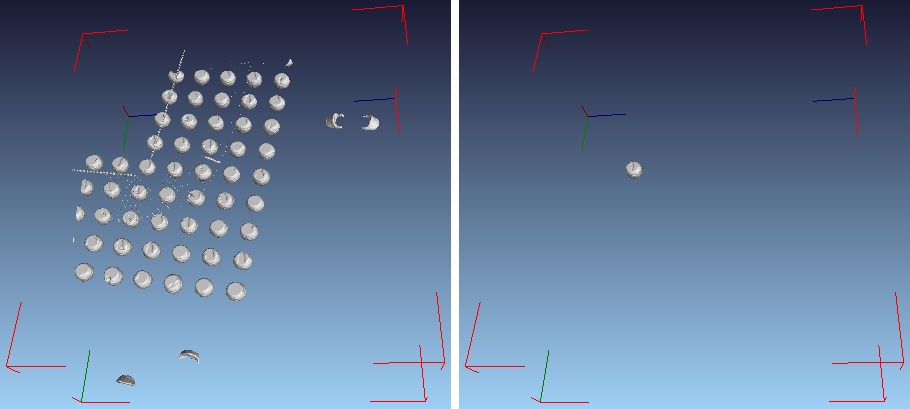
\includegraphics[width=0.9\textwidth]{RANSACball.png}
    \caption{In einem per Threshhold-Verfahren vorverarbeiteten Datensatz wird anhand eines einfachen Modells eine Kugel identifiziert.}
    \label{fig:ransac2}
  \end{center}
\end{figure}

\subsection{Bewertung}
Der Algorithmus eignet sich sehr gut um in großen Datenmengen schnell Instanzen von Modellen zu finden. Für den diskutierten Anwendungsfall ist er leider vergleichsweise langsam. Der Grund dafür ist, dass die zu suchenden Objekte schon durch einen Dichte-Threshhold sehr gut vor-isoliert werden können. Man kann sich deshalb direkt darauf konzentrieren einzelne Punktmengen auf bestimmte Eigenschaften hin zu untersuchen. Der große Vorteil von RANSAC schnell mögliche Kandidaten zu entdecken wird deshalb negiert.

\subsection{Alternativer Algorithmus zur Erkennung von Lötkugeln und Bonddrähten}
Der wohl am naheliegenste Ansatz Objekte in einem Datensatz zu finden, ist den Datensatz in einem hinreichend kleinen Raster abzusuchen und an jedem Punkt das damit verbundene Objekt auf die Ähnlichkeit mit den gesuchten Objekten zu betrachten.
Ein solcher Ansatz ist insbesonere bei den großen und einigermaßen wohlgeformten Lötkugeln sehr intuitiv, wie in der folgenden Abbildung zu sehen ist.


\begin{figure}[H]
  \begin{center}
    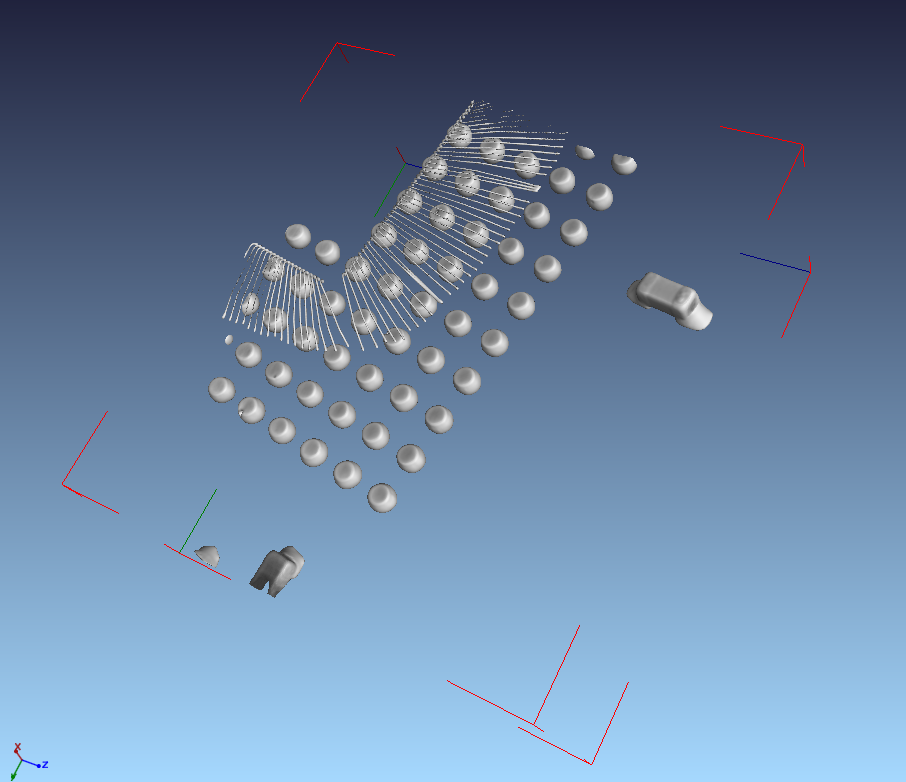
\includegraphics[width=0.9\textwidth]{BallsAndStuff.png}
    \caption{Die gesuchten Kugels sind hier ab einem bestimmten Reflektions-Schwellwert sehr einfach zu identifizieren, die Bonddrähte sind dagegen eher schwierig unter einen Hut zu bringen.}
    \label{fig:BallsAndStuff}
  \end{center}
\end{figure}

Das Vorgehen  bei einem solchen Algorithmus zur Suche der gezeigten Lötkugeln könnte also im einfachen Fall wie folgt aussehen:
\newline
%\begin{Algorithmus}
%\caption{Algorithmus in Pseudocode}
%\label{alg:sample}
\begin{algorithmic}
\Procedure{FindSpheres}{int $radius$, 3DUniformVoxelgrid g}
\State $searchStep = int(\sqrt{2} \cdot radius)$
\ForAll{Voxel $v \in g$ \bf{by Step} $searchStep$} \Comment \textnormal{Kurzform für die 3 Schleifen.} 
   \State $value = getValue(v)$
   \If{$value > 40000$}
       \If{$v \notin investigated$}
           \State $res = getFloodfill3D(v, value, tolerance = 8000)$
           \State $investigated = investigated \cup res$
           \State \bf{if} $isApproxSpheric(res.min, res.max)$ \bf{then} $found = found \cup res$  
       \EndIf
   \EndIf
\EndFor
\EndProcedure \newline
\end{algorithmic}
%\end{Algorithmus}

Hierbei sei als einfache Approximation nachfolgender Check gegeben (ggf. sollten hier Ansätze gewählt werden, die etwas durchdachter sind):
\newline
%\begin{Algorithmus}
%\caption{Algorithmus in Pseudocode}
%\label{alg:sample}
\begin{algorithmic}
\Procedure{isApproxSpheric}{int $min$, int $max$}
\State \bf{if} $max[1] \lor max[2] \lor max[3] = 0$ \bf{then return} \textnormal{False}
\State $xy = 0.65 < |min[0]-max[0]|/|min[1]-max[1]| < 1.35$
\State $xz = 0.65 < |min[0]-max[0]|/|min[2]-max[2]| < 1.35$
\State $zy = 0.65 < |min[2]-max[2]|/|min[1]-max[1]| < 1.35$
\State \bf{return} $xy \land xz \land zy$ \Comment \textnormal{Näherungsweise von "minimalem" Kubus umschlossen.}
\EndProcedure \newline
\end{algorithmic}
%\end{Algorithmus}

Für die Suche nach Bonddrähten reicht es, im obigen Algorithmus die Schrittweite, den Schwellwert und den Aproximationscheck zu ersetzen. Letzterer könnte im einfachen Fall beispielsweise wie folgt aussehen:
\newline
%\begin{Algorithmus}
%\caption{Algorithmus in Pseudocode}
%\label{alg:sample}
\begin{algorithmic}
\Procedure{isLongEnough}{int $min$, int $max$}
\State \bf{return} $40 < \sqrt{|min[0]-max[0]|^2 + |min[1]-max[1]|^2 + |min[2]-max[2]|^2}$
\EndProcedure \newline
\end{algorithmic}
%\end{Algorithmus}

Wie in nachfolgender Abbildung zu sehen ist, kann selbst ein derart einfacher Test reichen um die, durch den Schwellwert ohnehin schon gefilterten Objekte, perfekt einzuschränken.

\begin{figure}[H]
  \begin{center}
    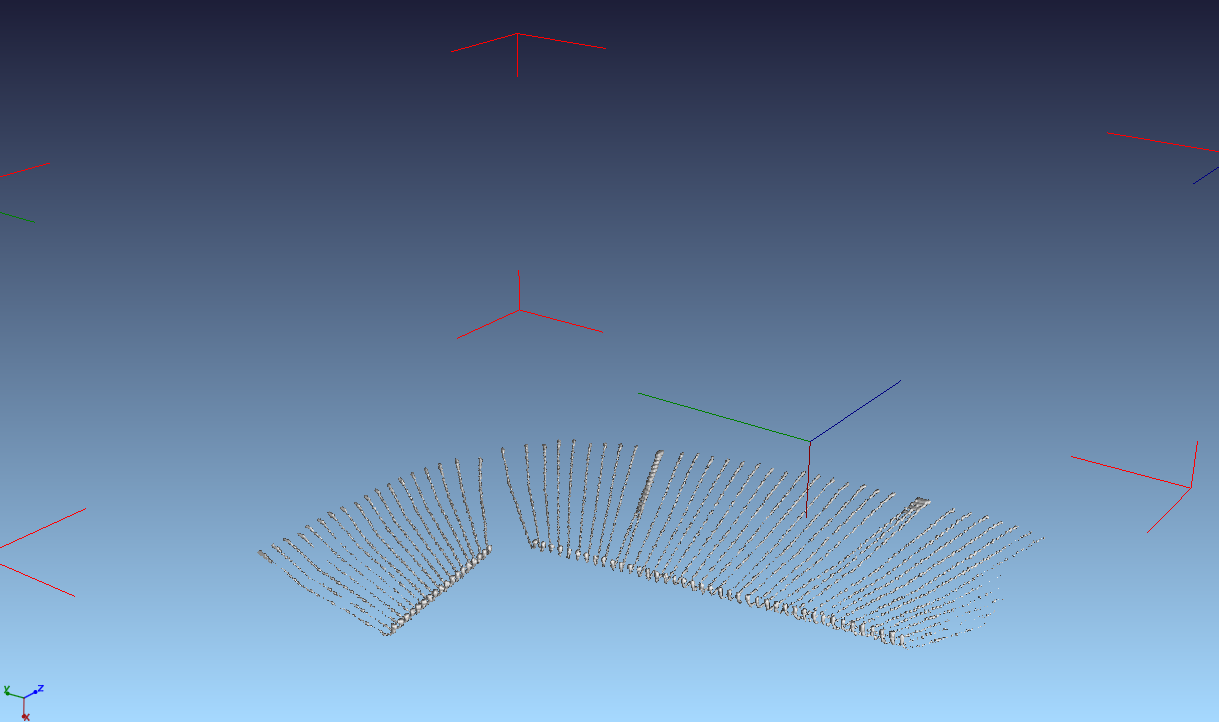
\includegraphics[width=0.9\textwidth]{Bond.png}
    \caption{Der Algorithmus erkennt im Beispieldatensatz alle Bonddrähte und Kugeln (hier nicht eingezeichnet). Durch die automatische Interpolation des Viewers sind die dargestellten Drähte etwas verwaschen.}
    \label{fig:Bond}
  \end{center}
\end{figure} 

\subsection{Bewertung}
Das Vorgehen des Algorithmus ist sehr intuitiv und einfach. Bei allen Tests reichten außerdem unkomplizierte Approximationsbedingungen, um die gesuchten und ausschließlich die gesuchten Objekte zu extrahieren.
Besonders einfach zu beschreibende geometrische Objekte, wie beispielsweise Kugeln, sind sehr einfach zu finden. \newline 
Um den Algorithmus auf ein Objekt zu eichen muss lediglich die Schrittweite und der Schwellwert angepasst werden und das vom Floodfill-Algorithmus zurückgegebene Objekt in den abschließenden Bedingungen hinreichend genau beschrieben werden. \newline
Ein Datensatz kann bei räumlich ausgedehnten Objekten schnell den Datensatz durchsuchen, da bei weitem nicht jeder Voxel untersucht werden muss (Bei Kugeln reicht beispielsweise eine Schrittweise von $\lfloor \sqrt{2} \cdot r \rfloor$). Die Geschwindigkeit ist selbstverständlich abhängig von der Größe und dem Vorkommen der gesuchten (und ähnlicher) Objekte.

